%%%
%
% $Autor: Malena Wilken $
% $Date: 2026-01-20 $
% $File: FlowchartDeployment.tex$
% $Version: 1 $
% !TeX spellcheck = en_US
% !TeX encoding = utf8
% !TeX root = filename 
% !TeX TXS-program:bibliography = txs:///biber
%
%%%%%%%%%%%%


\chapter{Tiny Machine Learning Kit} \label{chapter:TinyMLKit}

The Tiny Machine Learning Kit, see figure \ref{fig:TinyMLKit}, is a hardware set designed to support the development and evaluation of embedded machine learning applications. At its core, the kit is built around the Arduino Nano 33 BLE Sense, which integrates a microcontroller and a range of onboard sensors as described in chapter \ref{nano}. To extend its sensing capabilities toward visual input, the kit includes an OV7675 camera module, see chapter \ref{OV7675}, which can be connected via a Arduino-compatible shield. This shield is described in section \ref{TinyMLShield}. It provides the necessary electrical interfaces to integrate the camera and additional peripherals into a single system. In addition to the hardware, the kit is complemented by external educational content in the form of three courses provided by Harvard University via edX \cite{Harvard:2025}. These courses cover fundamental concepts of classical machine learning as well as the development and deployment of lightweight neural networks on embedded systems using TensorFlow Lite Micro \cite{ArduinoTinyMLKit:2022}.

\begin{figure}[H]
    \centering
    
\includegraphics[width=0.9\textwidth]{Nano33BLESense/TinyMLKit/TinyMachineLearningKit.png}
    \caption[Tiny Machine Learning Kit]{Tiny Machine Learning Kit \cite{ArduinoKit:2022}}
    \label{fig:TinyMLKit}
\end{figure}


\section{The Arduino Tiny Machine Learning Shield}
\label{TinyMLShield}

The TinyML Shield is a carrier and interface board designed to extend the Arduino Nano 33 BLE Sense with the camera OV7675, additional to connectivity and peripherals.

\begin{center}
	
	\begin{tikzpicture}
		\ArduinoNanoShieldTikz
	\end{tikzpicture}    
	
	\captionof{figure}[The Tiny Machine Learning Shield]{The Tiny Machine Learning Shield \cite{ArduinoShield:2021}}
	\label{fig:TinyMLShield}
\end{center}


The shield integrates the Arduino Nano via pin headers, outlined in figure \ref{fig:TinyMLShieldPinsArduino}, exposing both analog and digital signals while preserving access to power, reset, and communication lines. Dedicated connectors on the shield provide interfaces for external modules, most notably the camera connection, see figure \ref{fig:TinyMLShieldPinsOV7675}, which routes data and control signals required for image acquisition. Additional header pins allow access to I²C and GPIO signals, enabling the attachment of further sensors or actuators via Grove Connectors \cite{Arduino:2021b}. The pin configuration for the Grove interfaces is labeled on the Tiny Machine Learning Shield, see figure \ref{fig:TinyMLShield}.


%%% Arduino Nano Location on Tiny ML Shield

\begin{center}
	
	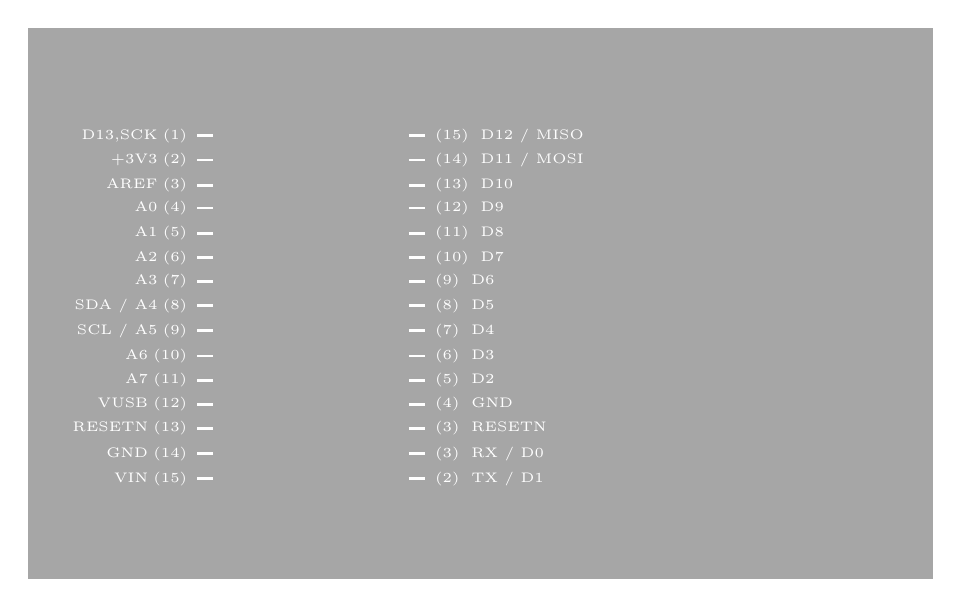
\begin{tikzpicture}
		\ArduinoNanoShieldTikz
		
		\fill[gray, opacity=0.7] (0,30) rectangle (11.5,23);
		
		
		\coordinate (A) at (2.34,29.03);
		\coordinate (B) at (7,19,23.81);   
		\coordinate (C) at (3.1,52.84);  
		\coordinate (D) at (4.1,28);  
	
		\begin{scope}
			\clip (2.34,29.03) rectangle (4.85,23.81);
			\ArduinoNanoShieldTikz
		\end{scope}
		
		\begin{scope}
			\clip (3.1,29.23) rectangle (4.1,28);
			\ArduinoNanoShieldTikz
		\end{scope}
			
		% --- Left Arduino Nano Header (Power + Analog) ---
		
		\node[left] at (2.15,28.63) {\textcolor{white}{\tiny D13,SCK\;(1)}};
		\draw[line width=1pt,white] (2.35,28.63) -- (2.15,28.63);
		
		\node[left] at (2.15,28.32) {\textcolor{white}{\tiny +3V3\;(2)}};
		\draw[line width=1pt,white] (2.35,28.32) -- (2.15,28.32);
		
		\node[left] at (2.15,28.00) {\textcolor{white}{\tiny AREF\;(3)}};
		\draw[line width=1pt,white] (2.35,28.00) -- (2.15,28.00);
		
		\node[left] at (2.15,27.71) {\textcolor{white}{\tiny A0\;(4)}};
		\draw[line width=1pt,white] (2.35,27.71) -- (2.15,27.71);
		
		\node[left] at (2.15,27.39) {\textcolor{white}{\tiny A1\;(5)}};
		\draw[line width=1pt,white] (2.35,27.39) -- (2.15,27.39);
		
		\node[left] at (2.15,27.08) {\textcolor{white}{\tiny A2\;(6)}};
		\draw[line width=1pt,white] (2.35,27.08) -- (2.15,27.08);
		
		\node[left] at (2.15,26.78) {\textcolor{white}{\tiny A3\;(7)}};
		\draw[line width=1pt,white] (2.35,26.78) -- (2.15,26.78);
		
		\node[left] at (2.15,26.47) {\textcolor{white}{\tiny SDA / A4\;(8)}};
		\draw[line width=1pt,white] (2.35,26.47) -- (2.15,26.47);
		
		\node[left] at (2.15,26.15) {\textcolor{white}{\tiny SCL / A5\;(9)}};
		\draw[line width=1pt,white] (2.35,26.15) -- (2.15,26.15);
		
		\node[left] at (2.15,25.83) {\textcolor{white}{\tiny A6\;(10)}};
		\draw[line width=1pt,white] (2.35,25.83) -- (2.15,25.83);
		
		\node[left] at (2.15,25.52) {\textcolor{white}{\tiny A7\;(11)}};
		\draw[line width=1pt,white] (2.35,25.52) -- (2.15,25.52);
		
		\node[left] at (2.15,25.215) {\textcolor{white}{\tiny VUSB\;(12)}};
		\draw[line width=1pt,white] (2.35,25.215) -- (2.15,25.215);
		
		\node[left] at (2.15,24.91) {\textcolor{white}{\tiny RESETN\;(13)}};
		\draw[line width=1pt,white] (2.35,24.91) -- (2.15,24.91);
		
		\node[left] at (2.15,24.59) {\textcolor{white}{\tiny GND\;(14)}};
		\draw[line width=1pt,white] (2.35,24.59) -- (2.15,24.59);
		
		\node[left] at (2.15,24.27) {\textcolor{white}{\tiny VIN\;(15)}};
		\draw[line width=1pt,white] (2.35,24.27) -- (2.15,24.27);
		
		
		% --- Right Arduino Nano Header (Digital + UART) ---
		
		\node[right] at (5.05,28.63) {\textcolor{white}{\tiny (15)\; D12 / MISO}};
		\draw[line width=1pt,white] (4.84,28.63) -- (5.05,28.63);
		
		\node[right] at (5.05,28.32) {\textcolor{white}{\tiny (14)\; D11 / MOSI}};
		\draw[line width=1pt,white] (4.84,28.32) -- (5.05,28.32);
		
		\node[right] at (5.05,28.00) {\textcolor{white}{\tiny (13)\; D10}};
		\draw[line width=1pt,white] (4.84,28.00) -- (5.05,28.00);
		
		\node[right] at (5.05,27.71) {\textcolor{white}{\tiny (12)\; D9}};
		\draw[line width=1pt,white] (4.84,27.71) -- (5.05,27.71);
		
		\node[right] at (5.05,27.39) {\textcolor{white}{\tiny (11)\; D8}};
		\draw[line width=1pt,white] (4.84,27.39) -- (5.05,27.39);
		
		\node[right] at (5.05,27.08) {\textcolor{white}{\tiny (10)\; D7}};
		\draw[line width=1pt,white] (4.84,27.08) -- (5.05,27.08);
		
		\node[right] at (5.05,26.78) {\textcolor{white}{\tiny (9)\; D6}};
		\draw[line width=1pt,white] (4.84,26.78) -- (5.05,26.78);
		
		\node[right] at (5.05,26.47) {\textcolor{white}{\tiny (8)\; D5}};
		\draw[line width=1pt,white] (4.84,26.47) -- (5.05,26.47);
		
		\node[right] at (5.05,26.15) {\textcolor{white}{\tiny (7)\; D4}};
		\draw[line width=1pt,white] (4.84,26.15) -- (5.05,26.15);
		
		\node[right] at (5.05,25.83) {\textcolor{white}{\tiny (6)\; D3}};
		\draw[line width=1pt,white] (4.84,25.83) -- (5.05,25.83);
		
		\node[right] at (5.05,25.52) {\textcolor{white}{\tiny (5)\; D2}};
		\draw[line width=1pt,white] (4.84,25.52) -- (5.05,25.52);
		
		\node[right] at (5.05,25.215) {\textcolor{white}{\tiny (4)\; GND}};
		\draw[line width=1pt,white] (4.84,25.215) -- (5.05,25.215);
		
		\node[right] at (5.05,24.91) {\textcolor{white}{\tiny (3)\; RESETN}};
		\draw[line width=1pt,white] (4.84,24.91) -- (5.05,24.91);
		
		\node[right] at (5.05,24.59) {\textcolor{white}{\tiny (3)\; RX / D0}};
		\draw[line width=1pt,white] (4.84,24.59) -- (5.05,24.59);
		
		\node[right] at (5.05,24.27) {\textcolor{white}{\tiny (2)\; TX / D1}};
		\draw[line width=1pt,white] (4.84,24.27) -- (5.05,24.27);
		

		
	\end{tikzpicture}    
	
	%    
\includegraphics[width=0.9\textwidth]{Nano33BLESense/TinyMLKit/TinyMachineLearningShieldRotated.png}
	\captionof{figure}[Pin Configuration of the Tiny Machine Learning Shield with Arduino Nano 33 BLE Sense]{Pin Configuration of the Tiny Machine Learning Shield with Arduino Nano 33 BLE Sense \cite{Arduino:2021b}}\label{fig:TinyMLShieldPinsArduino}
\end{center}


\begin{center}
    
    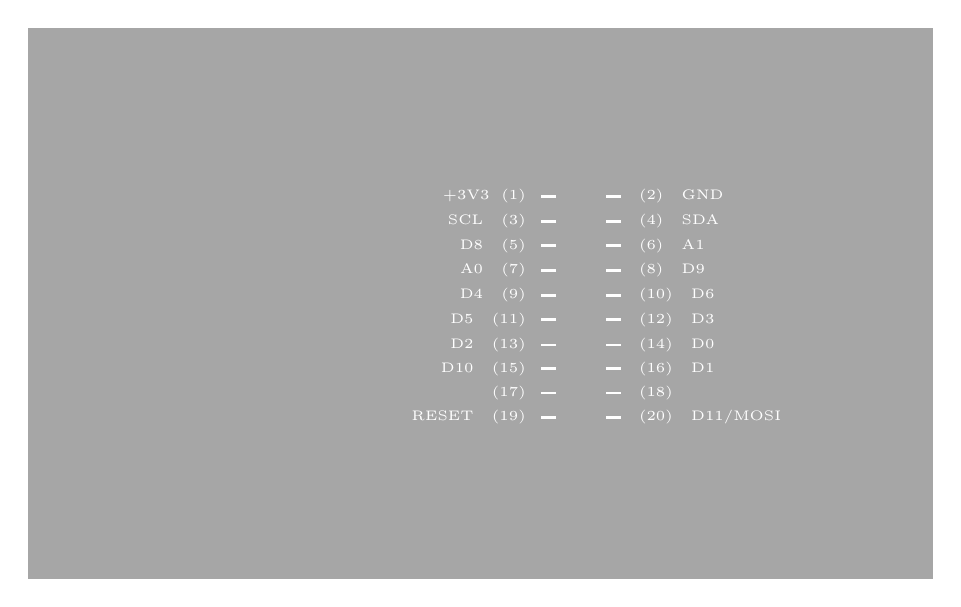
\begin{tikzpicture}
        \ArduinoNanoShieldTikz
        
        \fill[gray, opacity=0.7] (0,30) rectangle (11.5,23);
        
        
        \coordinate (A) at (6.61,28.14);
        \coordinate (B) at (7.45,24.81);    
        \begin{scope}
            \clip (A) rectangle (B);
            
            \ArduinoNanoShieldTikz
            
        \end{scope}
        
        
        %   \fill[black] (6.76, 27.97) rectangle (6.95, 27.76);
        \node[left]  at (6.45,27.86) {\textcolor{white}{\tiny +3V3 \;(1)}};
        \draw[line width=1pt,white] (6.71,27.86) -- (6.52,27.86);
        
        %   \fill[black] (7.09, 27.96) rectangle (7.29, 27.76);
        \node[right] at (7.64,27.86) {\textcolor{white}{\tiny (2) \; GND}};
        \draw[line width=1pt,white] (7.35,27.86) -- (7.54,27.86);
        
        %   \fill[black] (6.76, 27.64) rectangle (6.95, 27.44);
        \node[left]  at (6.45,27.54) {\textcolor{white}{\tiny SCL \; (3)}};
        \draw[line width=1pt,white] (6.71,27.54) -- (6.52,27.54);
        
        %   \fill[black] (7.1, 27.63) rectangle (7.29, 27.44);
        \node[right] at (7.64,27.54) {\textcolor{white}{\tiny (4) \; SDA}};
        \draw[line width=1pt,white] (7.35,27.54) -- (7.54,27.54);
        
        %   \fill[black] (6.77, 27.33) rectangle (6.96, 27.13);
        \node[left]  at (6.45,27.23) {\textcolor{white}{\tiny D8 \; (5)}};
        \draw[line width=1pt,white] (6.71,27.23) -- (6.52,27.23);
        
        %   \fill[black] (7.1, 27.32) rectangle (7.29, 27.13);
        \node[right] at (7.64,27.23) {\textcolor{white}{\tiny (6) \; A1}};
        \draw[line width=1pt,white] (7.35,27.23) -- (7.54,27.23);
        
        %   \fill[black] (6.76, 27.02) rectangle (6.96, 26.82);
        \node[left]  at (6.45,26.92) {\textcolor{white}{\tiny A0 \; (7)}};
        \draw[line width=1pt,white] (6.71,26.92) -- (6.52,26.92);
        
        %   \fill[black] (7.1, 27.01) rectangle (7.29, 26.82);
        \node[right] at (7.64,26.92) {\textcolor{white}{\tiny (8) \; D9}};
        \draw[line width=1pt,white] (7.35,26.92) -- (7.54,26.92);
        
        %   \fill[black] (6.77, 26.7) rectangle (6.96, 26.5);
        \node[left]  at (6.45,26.60) {\textcolor{white}{\tiny D4 \; (9)}};
        \draw[line width=1pt,white] (6.71,26.60) -- (6.52,26.60);
        
        %   \fill[black] (7.1, 26.7) rectangle (7.29, 26.5);
        \node[right] at (7.64,26.60) {\textcolor{white}{\tiny (10) \; D6}};
        \draw[line width=1pt,white] (7.35,26.60) -- (7.54,26.60);
        
        %   \fill[black] (6.77, 26.39) rectangle (6.96, 26.19);
        \node[left]  at (6.45,26.29) {\textcolor{white}{\tiny D5 \; (11)}};
        \draw[line width=1pt,white] (6.71,26.29) -- (6.52,26.29);
        
        %   \fill[black] (7.11, 26.38) rectangle (7.3, 26.19);
        \node[right] at (7.64,26.29) {\textcolor{white}{\tiny (12) \; D3}};
        \draw[line width=1pt,white] (7.35,26.29) -- (7.54,26.29);
        
        %   \fill[black] (6.76, 26.08) rectangle (6.96, 25.87);
        \node[left]  at (6.45,25.97) {\textcolor{white}{\tiny D2 \; (13)}};
        \draw[line width=1pt,white] (6.71,25.97) -- (6.52,25.97);
        
        %   \fill[black] (7.1, 26.07) rectangle (7.29, 25.87);
        \node[right] at (7.64,25.97) {\textcolor{white}{\tiny (14) \; D0}};
        \draw[line width=1pt,white] (7.35,25.97) -- (7.54,25.97);
        
        %   \fill[black] (6.76, 25.77) rectangle (6.95, 25.57);
        \node[left]  at (6.45,25.67) {\textcolor{white}{\tiny D10 \; (15)}};
        \draw[line width=1pt,white] (6.71,25.67) -- (6.52,25.67);
        
        %   \fill[black] (7.1, 25.76) rectangle (7.29, 25.57);
        \node[right] at (7.64,25.67) {\textcolor{white}{\tiny (16) \; D1}};
        \draw[line width=1pt,white] (7.35,25.67) -- (7.54,25.67);
        
        %   \fill[black] (6.76, 25.46) rectangle (6.95, 25.26);
        \node[left]  at (6.45,25.36) {\textcolor{white}{\tiny (17)}};
        \draw[line width=1pt,white] (6.71,25.36) -- (6.52,25.36);
        
        %   \fill[black] (7.1, 25.45) rectangle (7.29, 25.26);
        \node[right] at (7.64,25.36) {\textcolor{white}{\tiny (18)}};
        \draw[line width=1pt,white] (7.35,25.36) -- (7.54,25.36);
        
        %   \fill[black] (6.76, 25.15) rectangle (6.96, 24.94);
        \node[left]  at (6.45,25.05) {\textcolor{white}{\tiny RESET \; (19)}};
        \draw[line width=1pt,white] (6.71,25.05) -- (6.52,25.05);
        
        %   \fill[black] (7.1, 25.14) rectangle (7.29, 24.94);
        \node[right] at (7.64,25.05) {\textcolor{white}{\tiny (20) \; D11/MOSI}};
        \draw[line width=1pt,white] (7.35,25.05) -- (7.54,25.05);
        
        
        
        
        
    \end{tikzpicture}    
    
    %    
\includegraphics[width=0.9\textwidth]{Nano33BLESense/TinyMLKit/TinyMachineLearningShieldRotated.png}
    \captionof{figure}[Pin Configuration of the Tiny Machine Learning Shield with the Camera OV7675]{Pin Configuration of the Tiny Machine Learning Shield with the Camera OV7675 \cite{ArduinoShield:2021}}\label{fig:TinyMLShieldPinsOV7675}
    \end{center}
    

\section{Push Button}

\begin{center}
	
	
\begin{tikzpicture}
		\ArduinoNanoShieldTikz
		
		\fill[gray, opacity=0.7] (0,30) rectangle (11.5,23);
		
		%\fill[darkgray] (0.33, 28.68) rectangle (1.98, 27.2);
		\coordinate (A) at (0.33,28.68);
		\coordinate (B) at (1.98,27.2);   
		
		\begin{scope}
			\clip (A) rectangle (B);
			\ArduinoNanoShieldTikz
		\end{scope}
	\end{tikzpicture}    
	
	\captionof{figure}[Push Button on the Tiny Machine Learning Shield]{Push Button on the Tiny Machine Learning Shield}
	\label{fig:TinyMLShield}
\end{center}

The push button labeled PB1, as visualized in the circuit diagram \ref{fig:PushButtonTinyMLKit}, is connected as a momentary digital input that directly interfaces with the microcontroller pin D13. Electrically, one side of the switch is tied to the D13 signal line, while the opposite side is connected to ground. In its unpressed state, the switch is open and D13 is electrically disconnected from ground. When the button is pressed, the switch closes and pulls the D13 line to ground, generating a logic-low level at the pin. As shown in the schematic, there is no discrete pull-up or pull-down resistor associated with this connection, meaning that the electrical state of D13 while the button is not pressed is undefined unless the microcontroller configures an internal pull-up resistor in software. In typical operation, D13 would therefore be configured as an input with the internal pull-up enabled, causing the pin to read logic high when the button is released and logic low when the button is pressed. The button itself is a normally open, non-latching tactile switch that produces a purely digital signal and has no inherent analog behavior. It does not interact with the reset circuitry and has no effect on system startup unless its state is explicitly evaluated by the application code.


\begin{figure}[h]
	\begin{center}
		\includegraphics[width=\textwidth]{TinyML/PushButtonTinyMLKit}
		\caption[Circuit of Push Button Integration on the Tiny ML Shield]{Circuit of Push Button Integration on the Tiny ML Shield \cite{Arduino:2021b}}
		\label{fig:PushButtonTinyMLKit}
	\end{center}
\end{figure} 

\subsection{Example Code Manual}
To test the Push button, the Arduino Nano 33 BLE Sense must be correctly inserted into the TinyML Shield. Once mounted, the board is connected to the host device using a USB Micro cable, which provides both power and the programming interface. Within the Arduino IDE, the appropriate board configuration must be selected by choosing Arduino Nano 33 BLE as the target board, and the corresponding COM port assigned to the connected device must be set. After configuring the development environment, the example code visualized in section \ref{ExampleCodePB} can be implemented, compiled, and uploaded to the microcontroller via the USB connection. Upon successful upload, the program is executed immediately, allowing the hardware behavior to be verified directly on the TinyML Shield.

\subsection{Example Code} \label{ExampleCodePB}
This example code is presented to interacting with the built-in pushbutton on the TinyML shield. The implementation demonstrates how a digital input from the onboard button can be read and processed by the microcontroller, and how this input is subsequently used to control the state of the built-in LED of the Arduino Nano 33 BLE Sense, as well as an output in the serial monitor that describes the state of the button. This example is intended as a minimal and accessible starting point for further TinyML-related experiments, allowing the behavior to be extended toward more complex event handling or integrated into larger application logic. Note that with this code the Button is addressed with pin D12, which was proven to work, but in the scematic the button pin seems to be D13.


\begin{center}
	\captionof{code}{Push Button Test}
	\lstinputlisting[style=all]{../../Code/TinyMLKit/TestButton/TestButton.ino}
	\label{lst:PushButtonTest}
\end{center}

